\documentclass[french]{article}

\usepackage[french]{babel}
\usepackage[utf8]{inputenc}

\usepackage[legalpaper, margin=1in]{geometry}

\usepackage{graphicx}

\usepackage{listings}
\usepackage{subfig}
\usepackage{hyperref}


\begin{document}
    \title{Lectures}
    \maketitle

    \section{Notes de lectures}
    \begin{table}[h]
        \begin{center}
        \begin{tabular}{|p{0.3\textwidth}|p{0.15\textwidth}|p{0.55\textwidth}|}
            \hline
            Papier & Catégorie & Notes \\
            \hline
            ON THE LOGIC OF THEORY CHANGE: PARTIAL MEET CONTRACTION AND REVISION FUNCTIONS \cite{alchourron_logic_1985}
            & 
            & Contraction : On rejette une proposition x qui était auparavant dans une théorie A. La difficulté est souvent de savoir quelles propositions doivent être rejetées en même temps que x pour assurer la théorie soit fermée sous conséquence logique. Révision : On ajoute à la théorie A une proposition x, inconsistente à la théorie, et on doit alors réviser la théorie pour retrouver sa consistance au vu de ce nouveau fait.
            Levi identity: if A -. x denotes the contraction of A by x, then the revision of A by x, denoted A +. x, can be defined as Cn((A -. x) U {x}), where Cn is a given consequence operation.
            Définit des critères que doit valider le résultat d'un opérateur de révision sur une knowledge base. \\
            \hline
            An architecture of selective forgetting \cite{euzenat_architecture_1991}
            &
            & S’intéresse aux cas où les données sont liées entre elles. On en oublie une, que pasa pour celles liées ?
            - Pour les backwards références, c’est compliqué. Si on oublie un fait qui a été inféré d’autre chose, on risque juste de le ré-inférer à l’infini puisque les causes sont encore présentes. On part donc du principe qu’on va uniquement oublier des choses de la base de faits originale avant inférence (initial knowledge).
            - Pour les forward références, deux cas : consolidation (conséquence devient axiome), ou abstraction, qui revient à mettre la donnée oubliée dans un état particulier (true ou false).  \\
            \hline
            On the difference between updating a knowledge base and revising it \cite{katsuno_difference_1991}
            &
            & Update : le monde change, on change donc la base de connaissance. Ex : « le salaire de Joe augmente de 5% ».
            Revision : 0n change qqc dans un monde qu’on pense statique. Exemple : un test qu’on pensait vrai s’avère faux.
            Une des grosses différences est qu’on considère pour la révision que le fait initial était une erreur à la base et n’aurait jamais dû être inclus dans la base de fait, alors que pour l’update c’est juste une évolution. Propose des postulats pour le résultat d'un update, différents (mais proches) de ceux de la révision.
            \\
            \hline
            Intentional Forgetting in Artificial Intelligence Systems: Perspectives and Challenges \cite{timm_intentional_2018}
            & 
            & Programme « Intentional Forgetting in organizations » : paradigme interdisciplinaire entre informatique et psychologie. 8 projets, dont 5 orientés IA.
            Site du programme: http://www.spp1921.de/index.html.en \\
            \hline
            Psychological perspective on intentional forgetting \cite{ellwart_psychological_2019}
            & 
            & Présente différentes théories de l’oubli, d’un point de vue psycho. Fait la distinction entre oubli intentionnel, et les autres formes d’oubli. Présente une vision à l’échelle de l’individu, ou des groupes, et fait un lien avec l’IA. \\
            \hline
            Experiments in cultural language evolution - Intro \cite{steels_experiments_2012}
            &
            & Donnes quelques propriétés du langage : expressive adequacy (être assez précis sur ce qu'on veut dire), cognitive effort (qu'il soit facile à dire, et à comprendre), learnability (possibilité de l'étendre à de nouveaux phénomènes e.g), social conformity (une certaine conformité pour permettre de se comprendre). Ces propriétés vont agir comme pression sélective pour l'émergence d'un langage. Présente le principe des "language games". Lire les autres chapitres pour avoir une meilleure idée des expériences. \\
            \hline
        \end{tabular}
    \end{center}
    \end{table}
    \newpage
    \begin{table}[ht!]
        \begin{center}
        \begin{tabular}{|p{0.3\textwidth}|p{0.15\textwidth}|p{0.55\textwidth}|}
            \hline
            
            Classification des mécanismes organisationnels dans les réseaux d’agents \cite{lacomme_classification_2009}
            & 
            & Propose une classification des mécanismes organisationnels pour les SMA, et donne pour chacun plusieurs exemples. Classification proposée :
            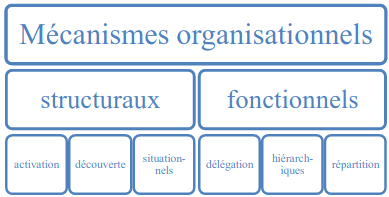
\includegraphics[width=8cm]{images/meca_orga.png}
            Peut être utile au moment de créer les jeux expérimentaux.
            \\
            \hline
            Une architecture d’agent BDI basée sur la théorie desfonctions de croyance : application à la simulation du comportement des agriculteurs \cite{taillandier_architecture_2012}
            &
            & Bon rappel avec exemple sur le fonctionnement des agents BDI, avec un exemple concret. \\
            \hline
            Intentional forgetting in distributed AI \cite{reuter_intentional_2019}
            &
            & Dans les cas où il faut bcp (trop) d'infos pour traiter un pb, les SMA vont souvent distribuer le problème afin de réduire sa complexité.
            Deux cas d'information overload (IO) : dimension qualitative, trop d'info car environnement trop riche -> agent spécialisés. Dimension quantitative, problème de la correspondance des informations, les agents peuvent s'échanger des infos fausses ou obsolètes -> bonne coordination.
            Compromis à trouver pour savoir commun : en avoir permet une meilleure coordo et + de redondance, moins de risque de perte de savoir utile, mais trop entraine des IO. 
            Principe de "team cognition", quand le savoir est partagé entre agents spécialisés. Team coalition : agents avec des capacités hétérogènes. Team formation : capacités homogènes. Du coup leur Intentional Forgetting sert + à une réorganisation du savoir.
            Les agents utilisés sont des "discourse agents", une variante de BDI.
            Pour définir les agents, on a l'ensemble des actions, et pour chaque agent un sous ensemble représentant les actions qu'il est autorisé à utiliser en fonction de son rôle dans l'équipe. En plus de BDI, les agents ont aussi un ensemble de plans "capability", représentant l'ensemble des plans qu'ils sont capables de réaliser.
            Une "transactive memory" permet de savoir qui est capable de quoi. Elle est individuelle, mais dans un monde idéal, tout le monde a une vision exacte des capacités de chacun, c'est donc un savoir partagé. Un modèle mental individuel également permet de savoir qui a quelles intentions. De la même manière, dans un monde parfait, il y a consensus là-dessus, et donc ce savoir individuel devient un savoir partagé.
            Quand un agent apprend ou oublie qqc, il suffit de le faire savoir à tlm pour qu'ils mettent leur TM à jour.
            \\
            \hline
            Description logics\cite{baader_chapter_2008}
            &
            & Analogie (personnelle, pas dans le papier), Tbox = classe, Abox = objet, instance. Dans le papier, Tbox = schema, Abox = data.
            Tbox est appelée "definitorial" ssi elle ne contient que des définitions, et qu'il n'y a pas de cycle.
            ALC une DL très utilisée, qui donne les bases, et a connu des extensions (par exemple "number restriction" pour ajouter des nombres à des définitions). Fait une comparaison entre DL, logique de 1er ordre et logique modale. A continuer.
            A noter (pas dans le papier) : le concept de "nominals" sort un peu du cadre Abox/Tbox, et peut permettre de faire référence aux datas au sein de la Tbox (par exemple qqn de telle classe doit forcément appartenir à telle asso, telle asso ou telle asso, sachant que les assos en question font partie de la Abox).
            \\
            \hline
            Towards Simulation-Based Role Optimization in Organizations \cite{reuter_towards_2017}
            &
            & Tente de résoudre le problème Job-Shop-Scheduling avec une approche multi-agent. Cherche avant tout à maximiser la répartition initiale des rôles, donc pas forcément utile pr moi, mais donne une bonne idée des objectifs de AdaptPro avec leur oubli intentionnel.\\
            \hline
        \end{tabular}
    \end{center}
    \end{table}
    \newpage
    \begin{table}[ht!]
        \begin{center}
        \begin{tabular}{|p{0.3\textwidth}|p{0.15\textwidth}|p{0.55\textwidth}|}

            \hline
            PR-OWL: A Bayesian Ontology Language for the Semantic Web \cite{da_costa_pr-owl_2008}
            &
            & Présente différentes alternatives bayésiennes. Les réseaux bayésiens classiques ne sont pas assez expressifs. L'approche proposée se base sur la logique MEBN (Multi Entity Bayesian Network), qui combine probas et logique de premier ordre. Certaines requêtes peuvent toutefois s'avérer indécidables. A continuer après + de recherches sur réseaux bayésiens\\
            \hline
            Bayesian Network \cite{pearl_bayesian_2011}
            &
            & Apprendre dans un tel réseau est un peu comme entrainer un NN : c'est faire varier les probas entre les entités (les poids des liens entre les noeuds). Un réseau causal est un réseau où les parents d'un noeud sont sa cause directe. Si on fixe la valeur d'un noeud, on retire alors le lien avec ses parents. Un peu vieux, donc probablement plus à jour, mais explique bien la base des réseaux bayésiens, et les idées derrière.
            \\
            \hline
            Advances in Bayesian network modelling: Integration of modelling technologies \cite{marcot_advances_2019}
            &
            & Présente de nombreux champs d'applications où des BN ont été utilisés. Peut être intéressant : agent based modeling. IBN, des BN intégrés à d'autres modèles. Ajd, ils sont surtout statiques (réalisés par des experts).
            \\
            \hline
            Bayesian or biased? Analytic thinking and political belief updating  \cite{tappin_bayesian_2020}
            & 
            & Etude de psycho cognitive. On pose des questions orientées politiquement à des personnes. Après chaque réponse, un signal indique vrai/faux. Ils ont été informés que ce signal donnait la bonne réponse 2 fois sur 3. On s'intéresse alors à comment les gens ont update leurs croyances, en leur posant les mêmes questions une seconde fois. Intéressant, mais se focalise surtout sur des idées polémiques, et donc des raisonnements motivés, pas des cas plus basiques. Etablit une corrélation (faible, mais significative statistiquement) entre score au RCT et capacité à update ses croyances en restant proche d'un modèle bayésien. Le test RCT peut en revanche être à creuser, illustre la capacité des individus à mobiliser + ou - de connaissances en fonction du contexte, rappelle le modèle "système 1 système 2" de Kahnemann, p-e un lien à faire avec oubli temporaire ?
            \\
            \hline
            Bayesian models of cognition \cite{l_griffiths_bayesian_2008}
            &
            & Cite au début bcp de modèles bayésiens utilisés en science cognitive, peut être utile. Un peu technique, mais présente différentes approches bayésiennes, dont les BNs, et leurs fondements mathématiques (surtout utile sur ce point).
            \\
            \hline
            Bayesian theories of conditioning in a changing world \cite{courville_bayesian_2006}
            &
            & Papier qui cite des études montrant que chez les animaux, la surprise (par exemple, conditionner l'animal à lui donner de la bouffe après une sonnerie, mais au bout d'un moment lui envoyer un choc électrique), et donne une interprétation bayésienne à ce fait (en gros, surprise -> grosse incertitude sur leurs croyances actuelles -> plus gros updates dans les probas de leurs croyances). A creuser, voir si ce mécanisme existe aussi pr l'oubli ? (si on oublie bcp de chose, ça peut vouloir dire que l'envt a bcp changé, donc entrainer moins de confiance dans nos connaissances actuelles et rendre l'oubli + probable ?). Direction à creuser.
            \\
            \hline

            The case for Motivated Reasonning \cite{kunda1990case}
            &
            & Présente le phénomène de "raisonnement motivé". Historiquement, une thèse concurrente était de dire que simplement, pour certains individus, certaines croyances étaient + plus plausibles au vu de leurs croyances initiales (prior believes) Peut être intéressant pour les oublis temporaires. (à continuer)
            \\
            \hline

            Revision in network of ontologies \cite{euzenat_revision_2015}
            & 
            & Commence par définir les propriétés d'un réseau d'ontologie. "Revision defines operators for modifying a theory (K) in the logic when some action occurs, like the knowledge that an assertion must be believed (revision), must not be believed (retraction), or does hold after a change (update). These operators are constrained by several postulates". Propose ensuite des opérateurs (dérivés de partial meet revision) pour de la révision dans un réseau d'ontologies.

            \\
            \hline
        \end{tabular}
    \end{center}
    \end{table}
    \newpage
    \begin{table}[ht!]
        \begin{center}
        \begin{tabular}{|p{0.3\textwidth}|p{0.15\textwidth}|p{0.55\textwidth}|}
            \hline
            The  Role  of  Forgetting  in  Learning \cite{marcot_advances_2019}
            &
            & Dans le cadre de résolution de problèmes, on peut quantifier l'utilité d'un savoir : on résout le problème avec ou sans ce savoir, et la différence donne une idée sur la pertinence de ce savoir. Un savoir avec une valeur négative peut être oublié.
            Toutefois, un savoir faux peut s'avérer mieux que pas de savoir du tout : penser que tous les grizzlis sont des mangeurs d'humain (savoir trop généralisé) > n'avoir aucune info sur leur dangerosité. Au contraire, des savoirs corrects peuvent entrainer à des erreurs (cite un papier). Mène ensuite des expériences sur de la recherche dans des graphes. Pas forcément hyper proche de ce que je fais, mais à garder en tête, peut-être creuser les aspects où au-delà d'être inutile, le savoir devient contre-productif, même si vrai. \\
            \hline

            Intentional Forgetting: An Emerging Field in AI and Beyond \cite{beierle_intentional_2019}
            &
            & Fait un point sur l'oubli intentionnel dans l'IA en présentant différents papiers/projets (surtout en lien avec le programme de recherche allemand, mais pas que, biblio à creuser).\\
            \hline
            

            A Description Logic Primer \cite{krotzsch_description_2013}
            &
            & Très bonne intro aux DL, clair. Ne pas hésiter à revenir dessus si besoin.
            \\
            \hline

            Processes of Successful Intentional Forgetting \cite{johnson_processes_1994}
            & 
            & Papier de psycho cognitive, qui propose un framework pour l'intentional forgetting. Intentional forgetting is defined as a motivated attempt to limit the future expression of aspecific memory content. This definition differs from that of spontaneous forgetting, which occurs without motivation and regardless of the information's validity or relevance.
            Fait une distinction entre les études où les sujets sont prévenus ou non sur le fait qu'il faudra oublier : cette info changera la manière dont ils vont encoder l'info. Dans le cas où ils le savent, on ne considère pas ça comme intentional forgetting.
            Fait une différence entre deux approches de traitement de l'IF : les processus "memory-based", par exemple l'inhibition d'une donnée au sein de la mémoire, ou la ségrégation, le fait d'avoir une donnée en mémoire, mais avec un "flag" indiquant qu'elle ne doit pas être prise en compte. De l'autre côté, les processus decision-based, qui eux vont agir sur le R-cued, le signal de rappel d'une donnée, et vont faire que ce signal va moins probablement renvoyer la donnée oubliée. Présente un framework tentant de regrouper toutes ces approches (papier ancien, peut-être plus à jour, voir les recherches + récentes).

            \\
            \hline

            A Brief Survey on Forgetting from a Knowledge Representation and Reasoning Perspective \cite{timm_intentional_2018}
            &
            & Utilise une déf un peu différente de processus d'oubli intentionnel, par exemple ne pas prendre en compte toutes nos connaissances pour résoudre un problème particulier est considéré comme oubli intentionnel. Pour eux, abstraction = red whine and white whine merged to whine.
            Logique propositionnelle, oubli de variables : semantic changes should affect only the forgotten variable p, càd que le résultat d'une interprétation avant/après oubli doit tjrs être le même pour au moins une interprétation de la valeur oubliée. Définit logiquement un tel oubli. Variable forgetting aims at eliminating any occurrence of a variable. A more fine‑grained extension considered by Lang et al. [60] is to forget literals, where an atom p and its negation not(p) are distinguished. Définit logiquement l'oubli de literals (en gros, oublier qu'une telle variable peut être vraie, ou fausse, et ne garder que les cas ou elle est fausse, ou vraie, exemple 9 illustre bien).
            Logique de premier ordre, oubli de faits, bien illustré exemple 12.
            Oubli de relation : par exemple si on veut oublier "student", et qu'on a "student(Jon), on va remplacer par "Il existe R tq R(John)", donnant une formule du second ordre (exemple 13).
            Enfin, oubli d'individu, via l'anonymisation : student(John) devient, après l'oubli de John, Il existe x tq student(x).
            Pour les DL, parle de la difficulté à oublier tout en conservant la similarité des modèles : c'est parfois impossible/indécidable. Cite de nombreuses réfs de travaux en lien avec l'oubli en DL. Parle ensuite d'oubli pour ASP et logiques modales.
            Evoque certaines raisons de l'oubli, par exemple variables indépendantes, qu'on peut supprimer sans que cela n'ait d'impact sur la KB.
            \\
            \hline


        \end{tabular}
    \end{center}
    \end{table}

    \section{Champs libre, notes en vrac}

    Regarder les recherches du laboratoire de psychologie et neurocognition

    Idées en vrac :
    Raisonnement motivé - cherry picking, variables indépendantes, système de Kahnemann...

    
    \nocite{*}
    \bibliographystyle{plain}
    \bibliography{bibli}
\end{document}